% Auto-generated multi-workload figure snippets.

\begin{figure}[t]
  \centering
  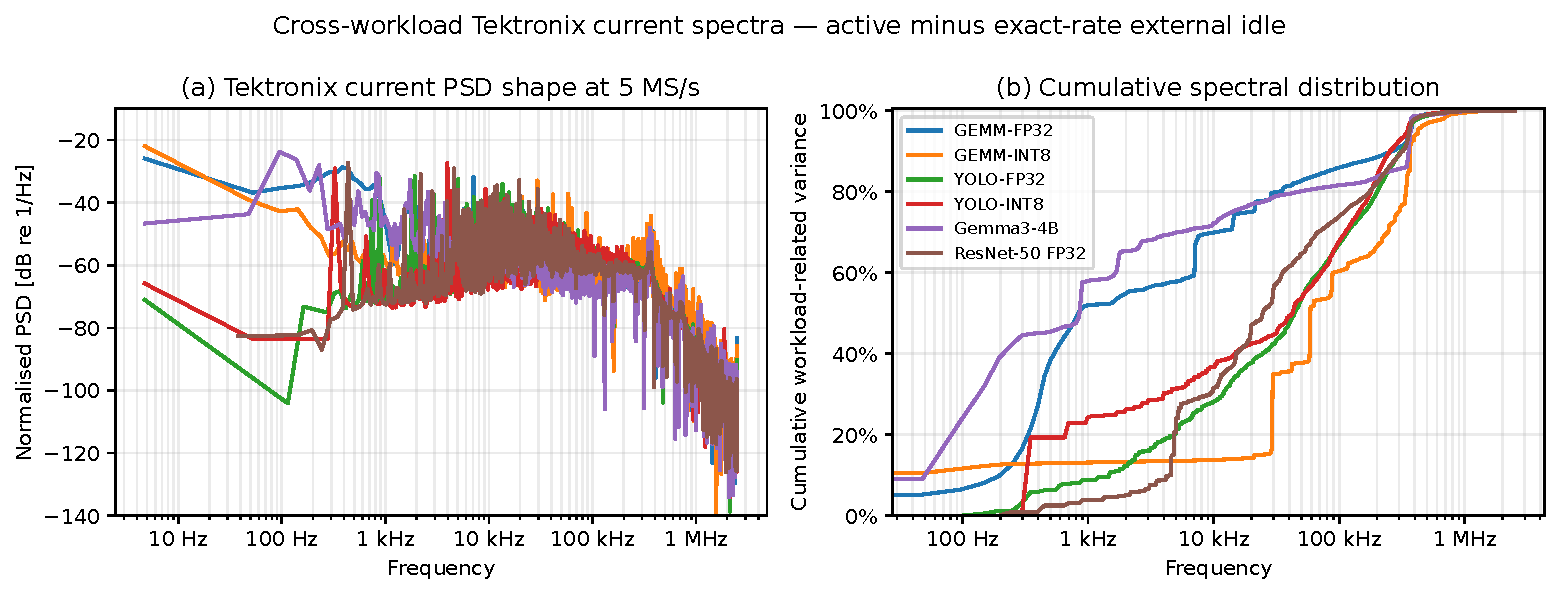
\includegraphics[width=\textwidth]{paper_artifacts/figures/cross_workload_current_psd_paper.pdf}
  \caption{Cross-workload Tektronix current spectra at the common 5-MS/s rate. Each curve subtracts the exact-rate external-idle median. The left panel shows the normalised PSD shape in dB relative to 1/Hz; the right panel shows the cumulative workload-related variance in percent.}
  \label{fig:cross-workload-current-psd}
\end{figure}

\begin{figure}[t]
  \centering
  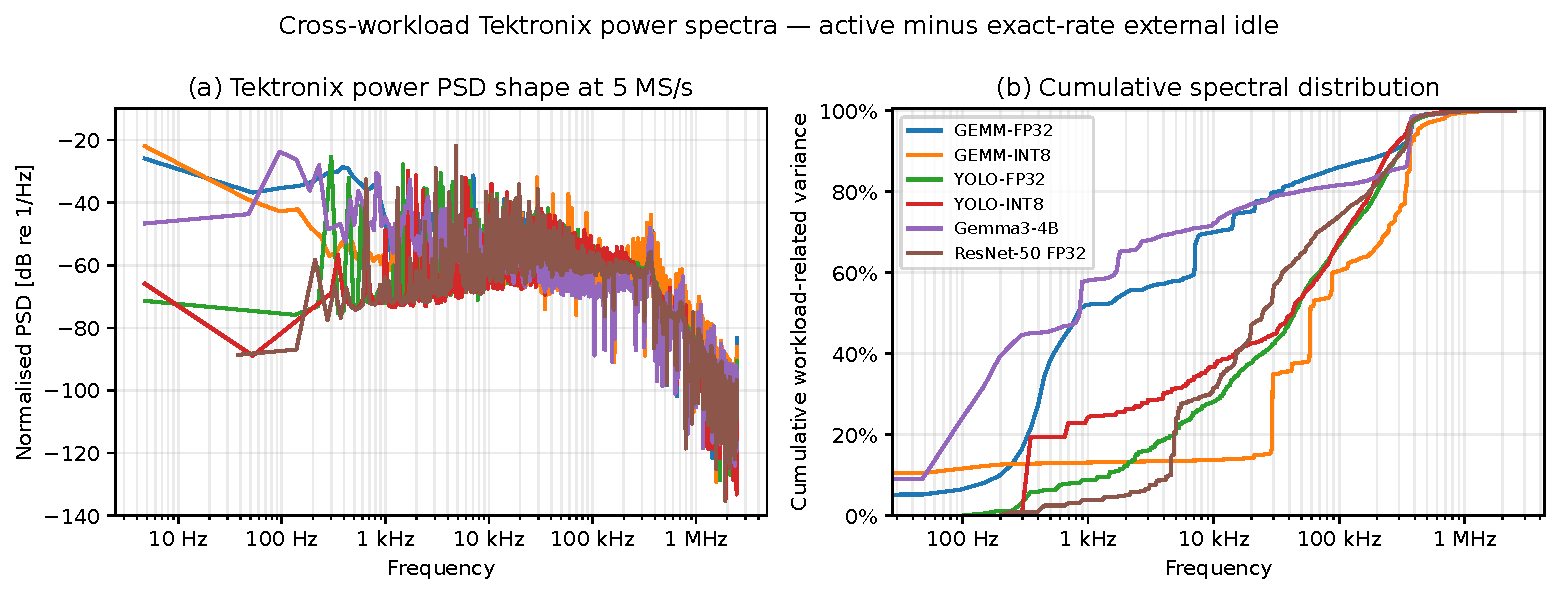
\includegraphics[width=\textwidth]{paper_artifacts/figures/cross_workload_power_psd_paper.pdf}
  \caption{Cross-workload spectra of estimated power derived from the calibrated current traces using the shared current-dependent voltage model. The left panel shows normalised PSD shape; the right panel shows cumulative workload-related power variance.}
  \label{fig:cross-workload-power-psd}
\end{figure}

\begin{figure}[t]
  \centering
  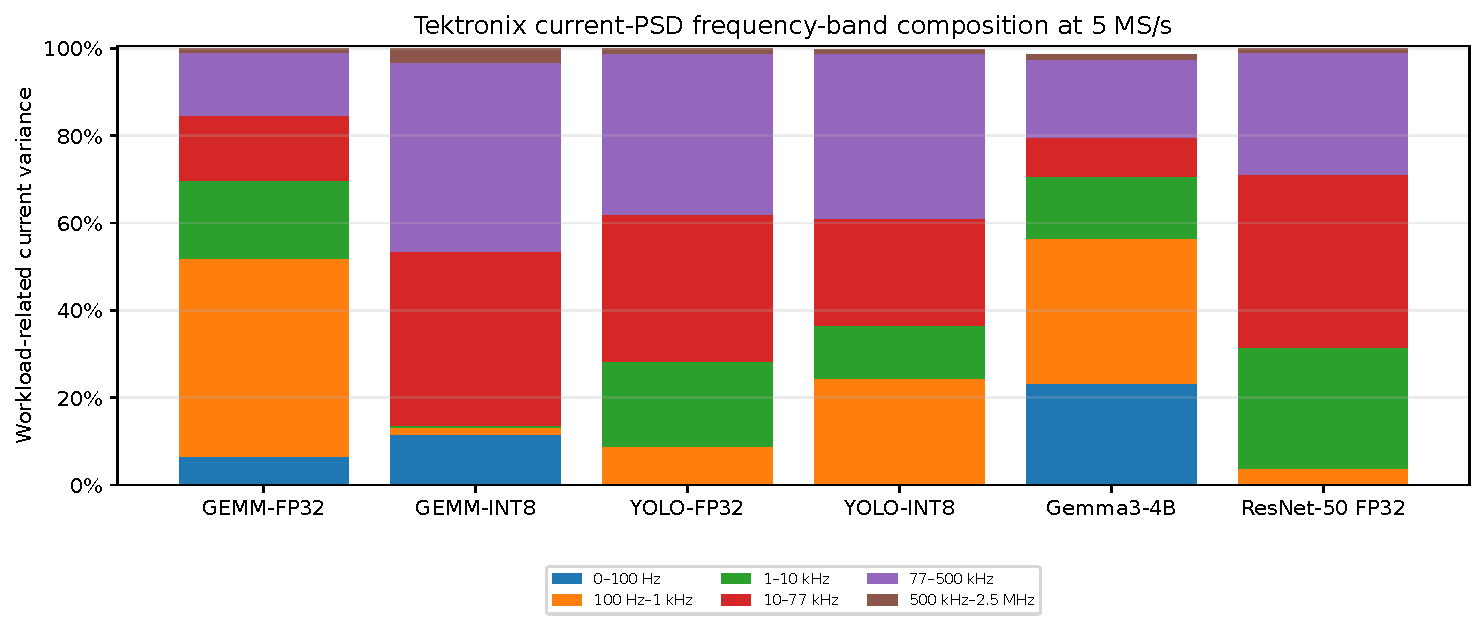
\includegraphics[width=\textwidth]{paper_artifacts/figures/cross_workload_frequency_bands_paper.pdf}
  \caption{Frequency-band composition of the workload-related Tektronix current variance at 5 MS/s.}
  \label{fig:cross-workload-bands}
\end{figure}

\begin{figure}[t]
  \centering
  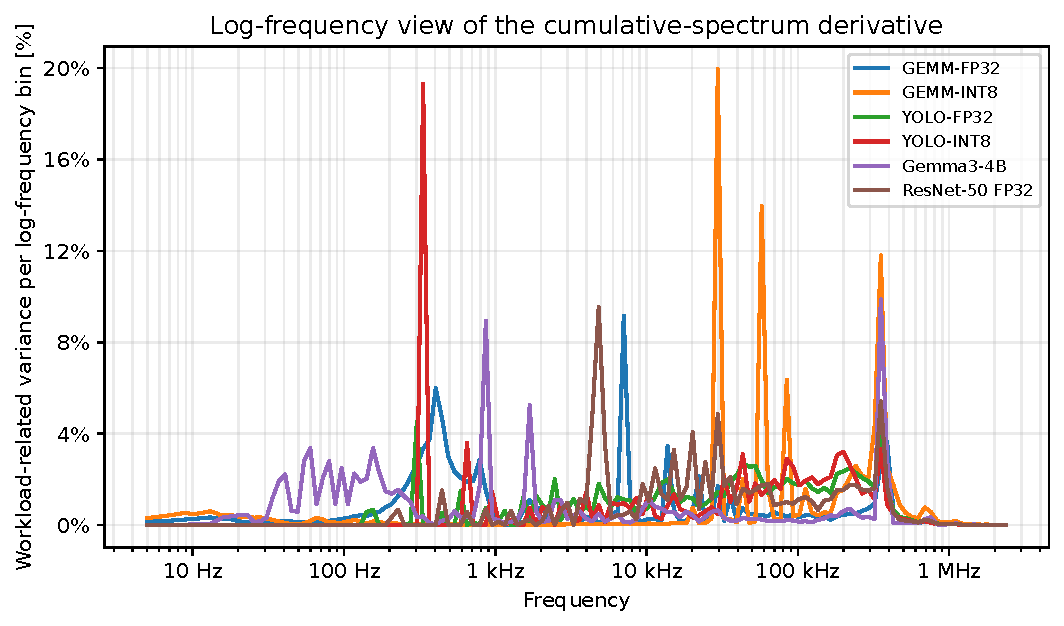
\includegraphics[width=\textwidth]{paper_artifacts/figures/cross_workload_log_frequency_variance_share_paper.pdf}
  \caption{Log-frequency view of the cumulative-spectrum derivative. Each point reports the workload-related variance share in one fixed-width logarithmic frequency bin; the shares sum to 100 percent across the analysed band.}
  \label{fig:cross-workload-log-derivative}
\end{figure}

\begin{figure}[t]
  \centering
  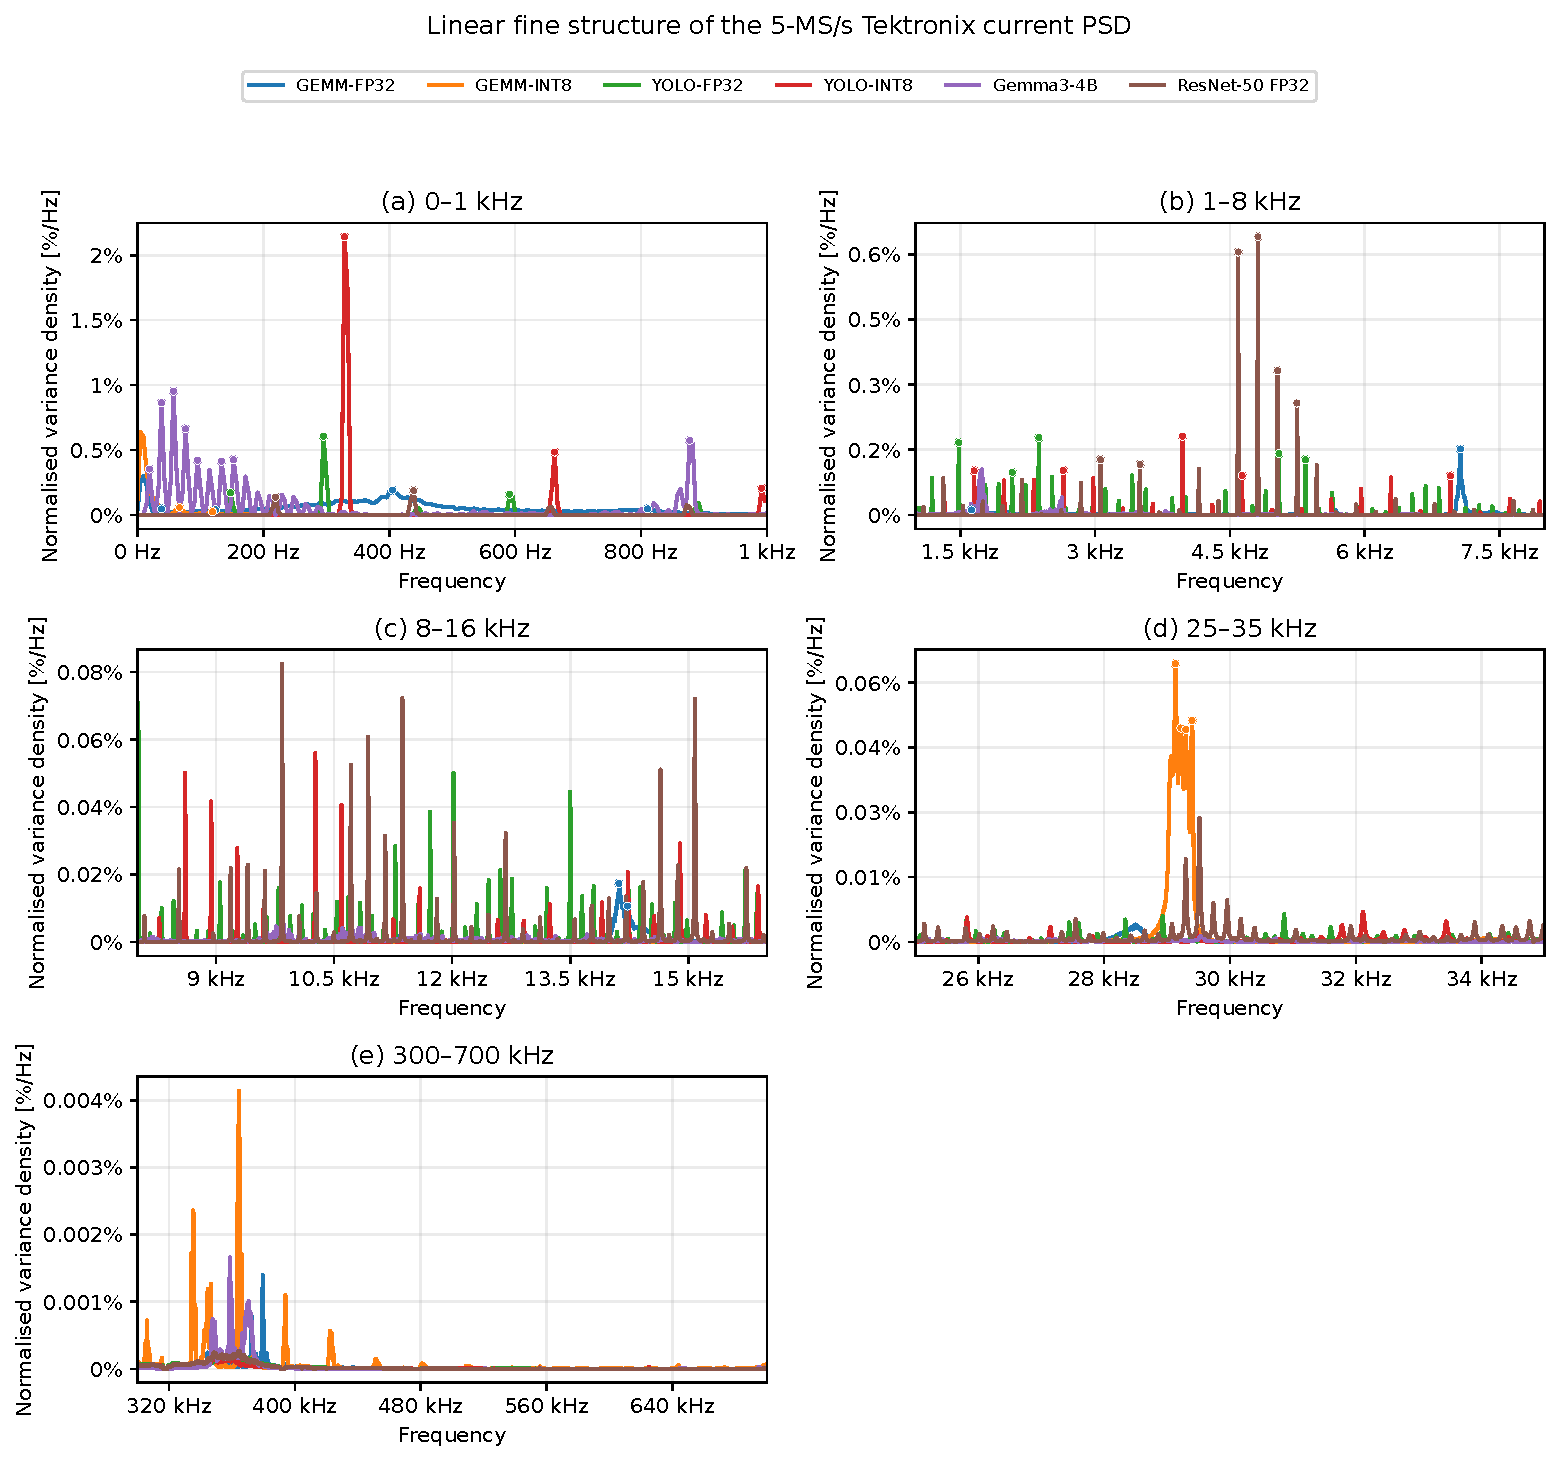
\includegraphics[width=\textwidth]{paper_artifacts/figures/cross_workload_psd_fine_structure_paper.pdf}
  \caption{Linear-axis fine structure of the normalised Tektronix current PSD in selected low-frequency, mid-frequency, precision-sensitive 25–35-kHz, and upper-tail regions. Exact dominant-peak frequencies remain listed in the generated CSV artifacts.}
  \label{fig:cross-workload-fine-structure}
\end{figure}

\begin{figure}[t]
  \centering
  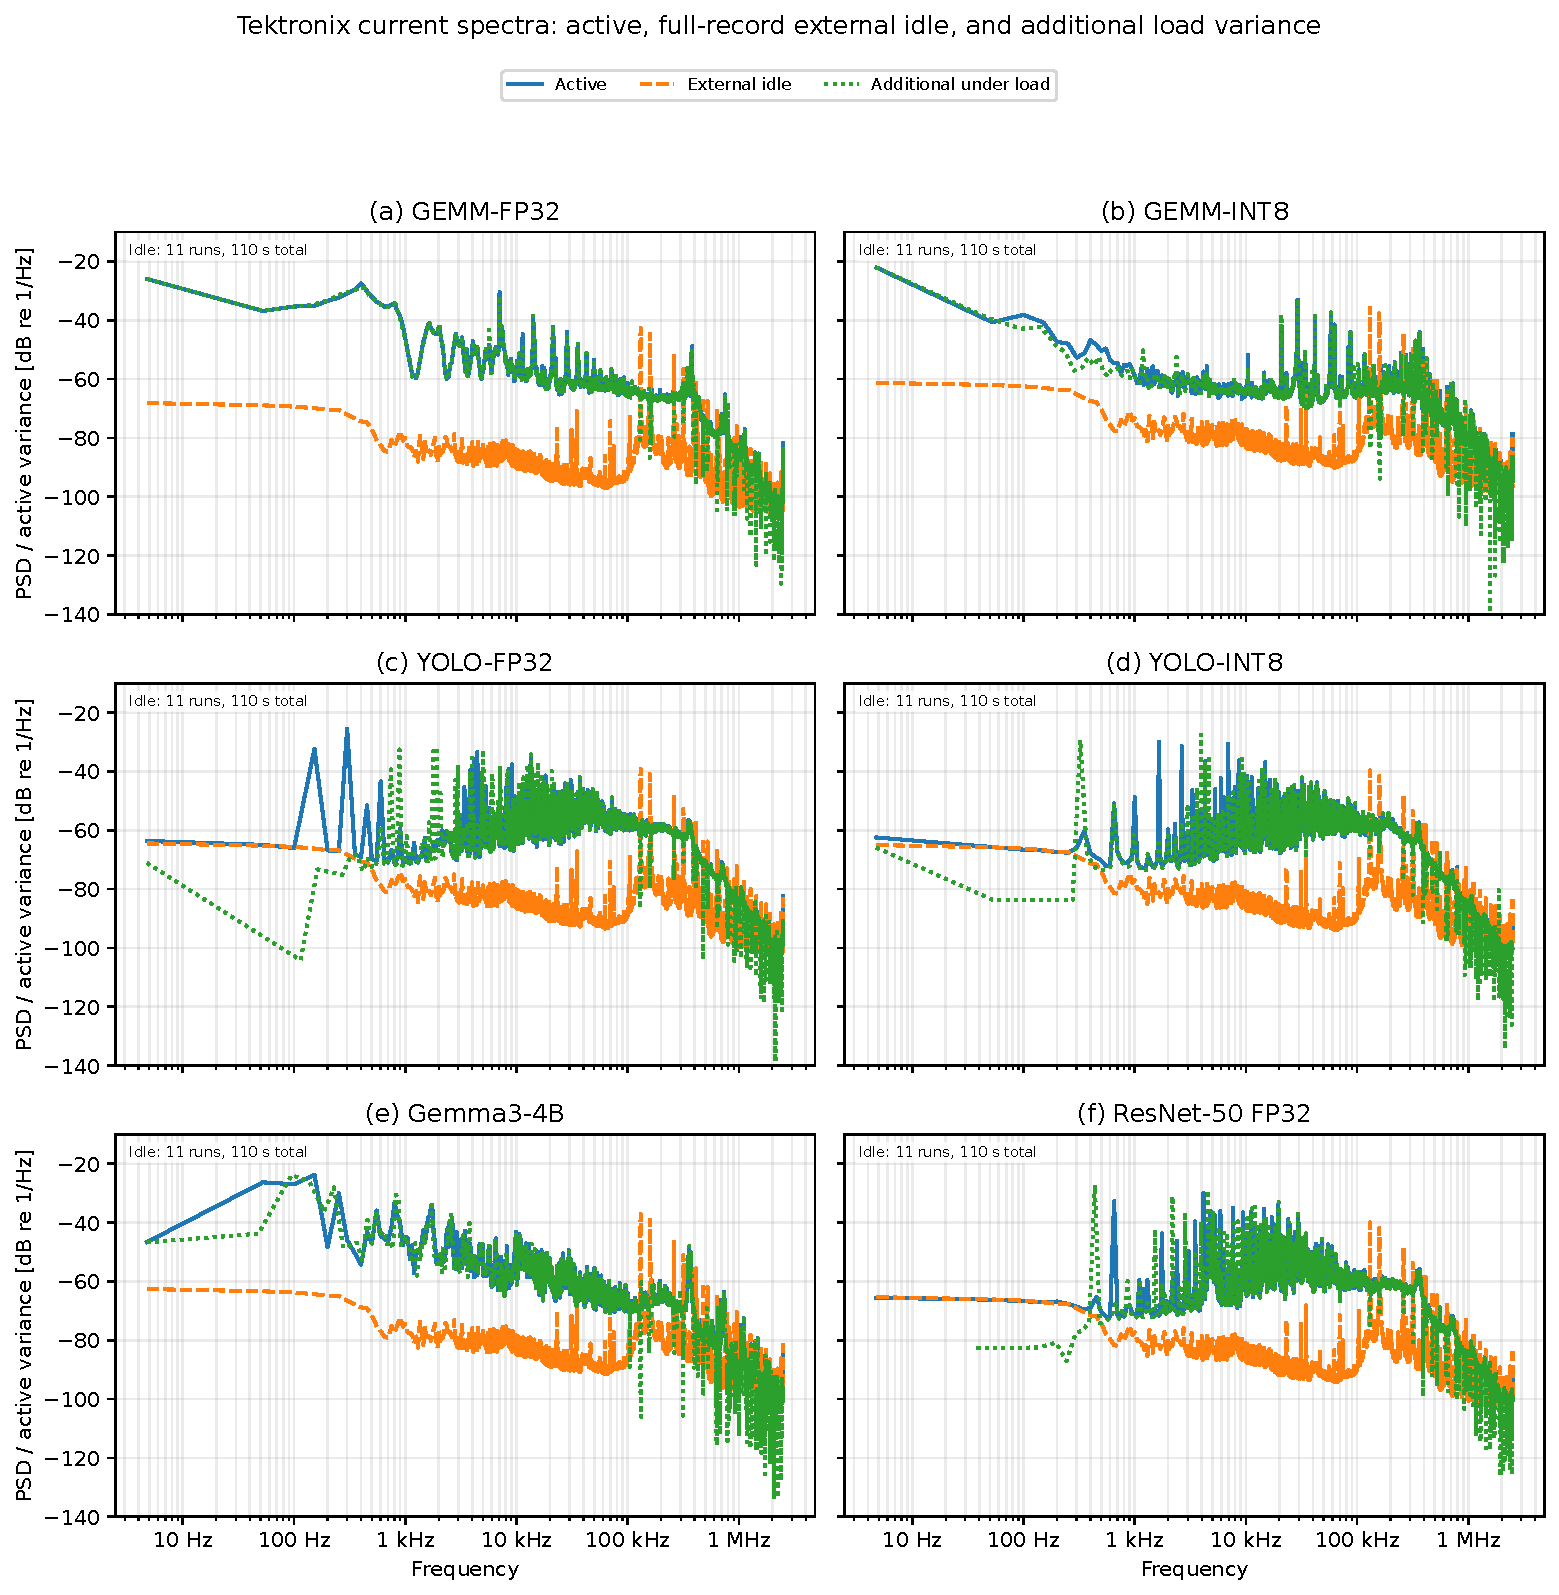
\includegraphics[width=\textwidth]{paper_artifacts/figures/cross_workload_active_idle_psd_paper.pdf}
  \caption{Per-workload Tektronix current spectra for active operation, full-record exact-rate external idle, and the additional under-load component max(active-idle,0). Every physical idle run is analysed at its full duration with the same Welch method; physical runs receive equal weight in the cross-run median.}
  \label{fig:cross-workload-active-idle}
\end{figure}

\begin{figure}[t]
  \centering
  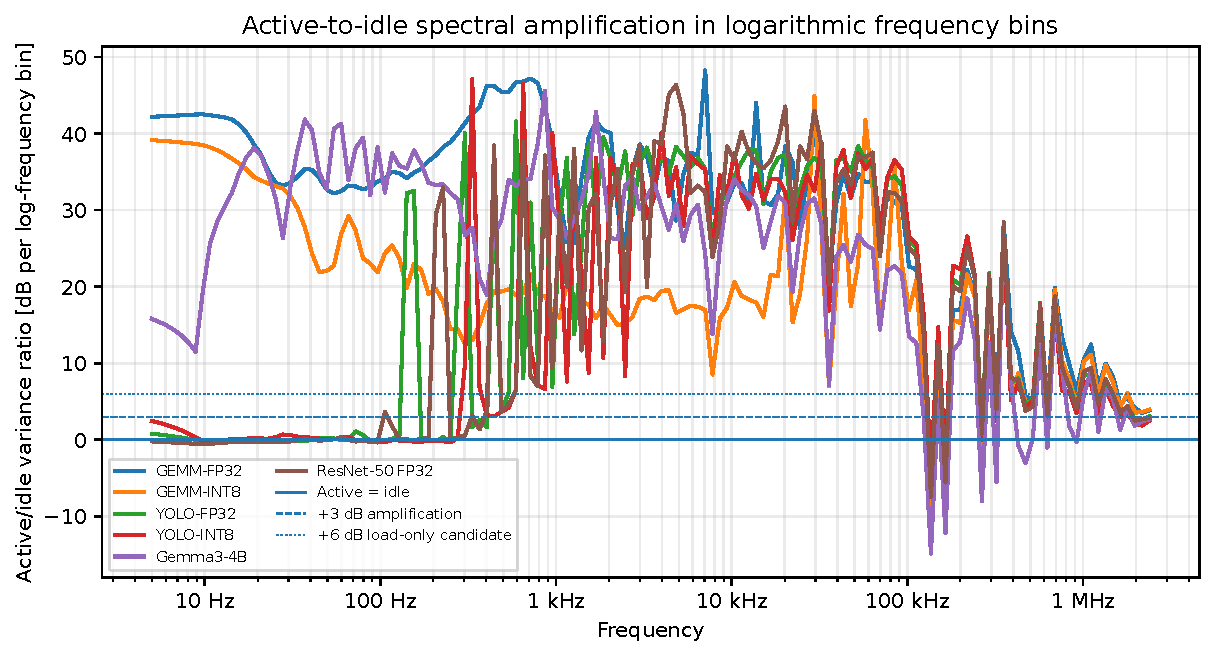
\includegraphics[width=\textwidth]{paper_artifacts/figures/cross_workload_active_idle_ratio_paper.pdf}
  \caption{Integrated active-to-idle Tektronix current-variance ratio in equal-width logarithmic frequency bins. Positive values indicate more variance under load; the 3-dB and 6-dB guide lines mark the configured load-amplified and load-only-candidate thresholds. Active and idle are independent acquisitions, so the comparison is descriptive rather than phase-coherent source separation.}
  \label{fig:cross-workload-active-idle-ratio}
\end{figure}

\begin{figure}[t]
  \centering
  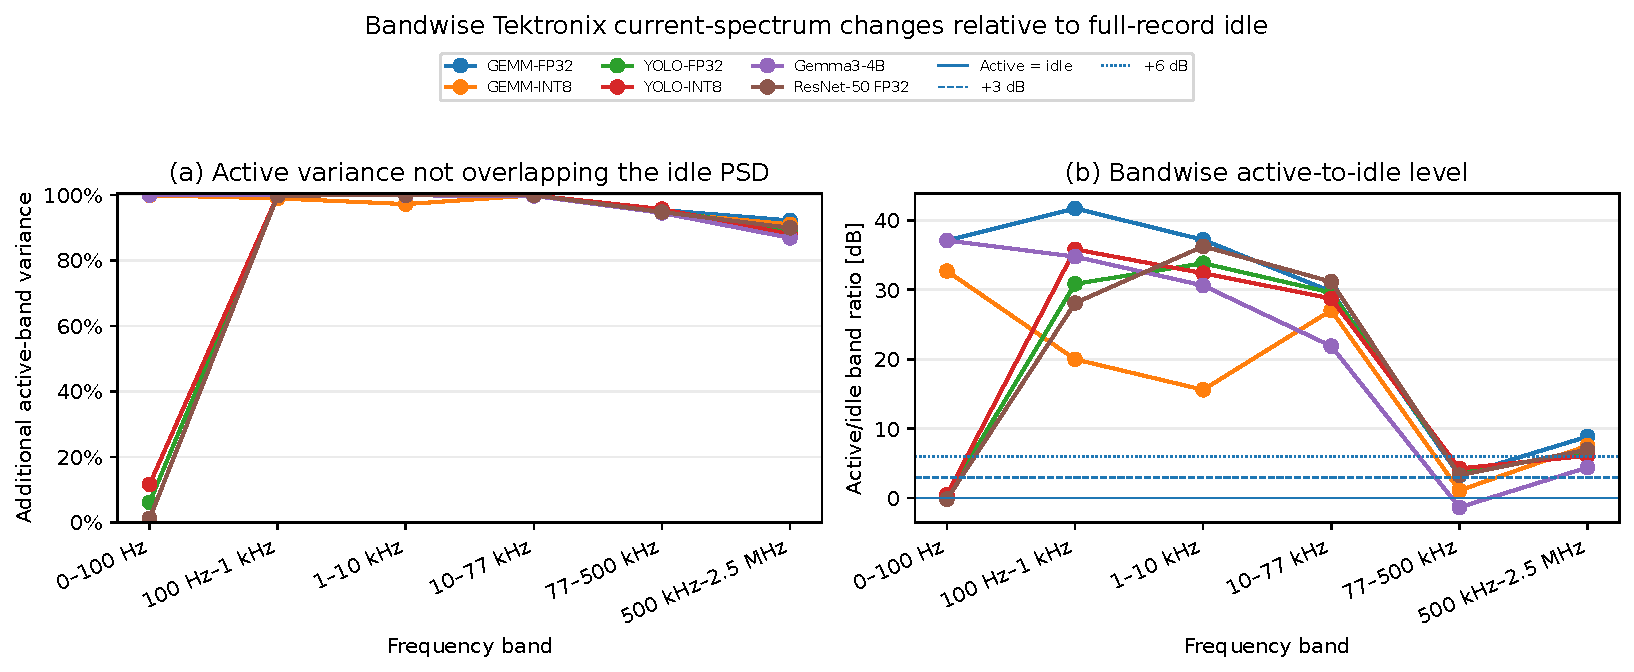
\includegraphics[width=\textwidth]{paper_artifacts/figures/cross_workload_idle_load_frequency_bands_paper.pdf}
  \caption{Bandwise comparison of active and external-idle Tektronix current spectra. Panel (a) shows the fraction of active-band variance that exceeds the idle PSD; panel (b) shows the integrated active/idle PSD ratio. This is a descriptive comparison of independent records, not phase-coherent source separation.}
  \label{fig:cross-workload-idle-load-bands}
\end{figure}

\begin{figure}[t]
  \centering
  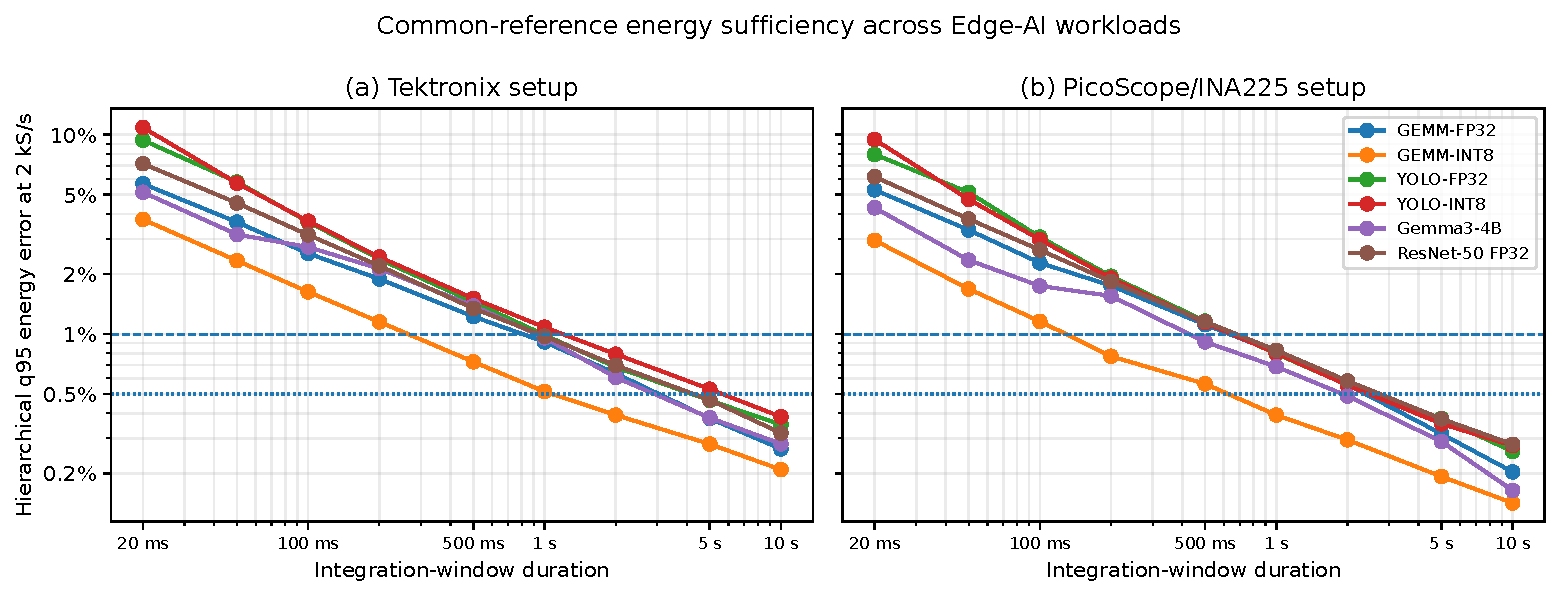
\includegraphics[width=\textwidth]{paper_artifacts/figures/cross_workload_energy_duration_paper.pdf}
  \caption{Duration-dependent common-reference energy error at 2 kS/s. Each point is the hierarchical q95: window-position and sampling-grid-offset sensitivity are first aggregated within each physical run and then across physical runs. The horizontal lines mark the 0.5% and 1% criteria.}
  \label{fig:cross-workload-duration}
\end{figure}

\begin{figure}[t]
  \centering
  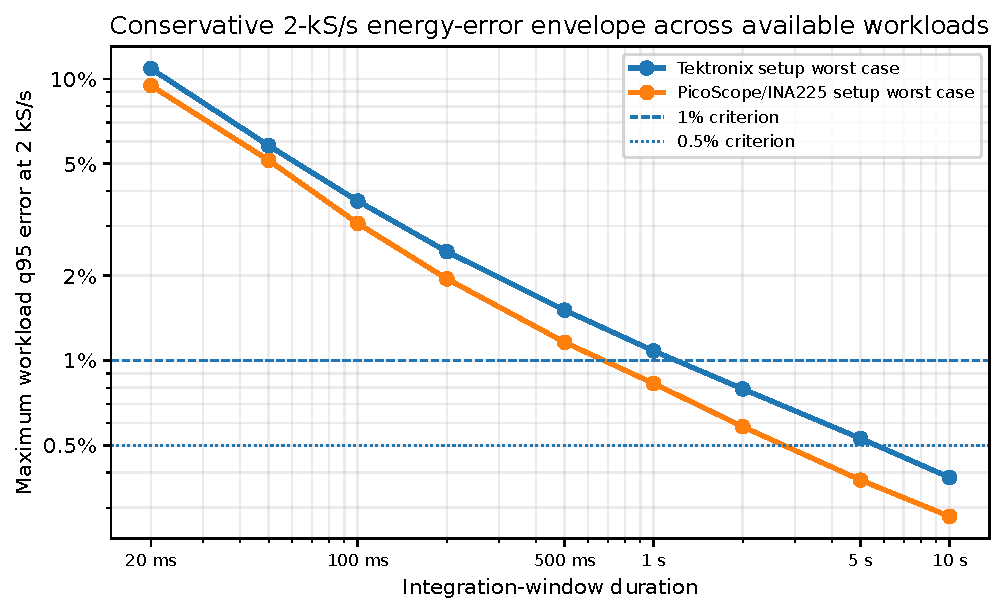
\includegraphics[width=\textwidth]{paper_artifacts/figures/cross_workload_worst_case_envelope_paper.pdf}
  \caption{Conservative worst-case 2-kS/s energy-error envelope. At each integration duration, the plotted value is the maximum hierarchical q95 among all currently available workloads; the horizontal lines mark the 0.5% and 1% criteria.}
  \label{fig:cross-workload-worst-envelope}
\end{figure}

\begin{figure}[t]
  \centering
  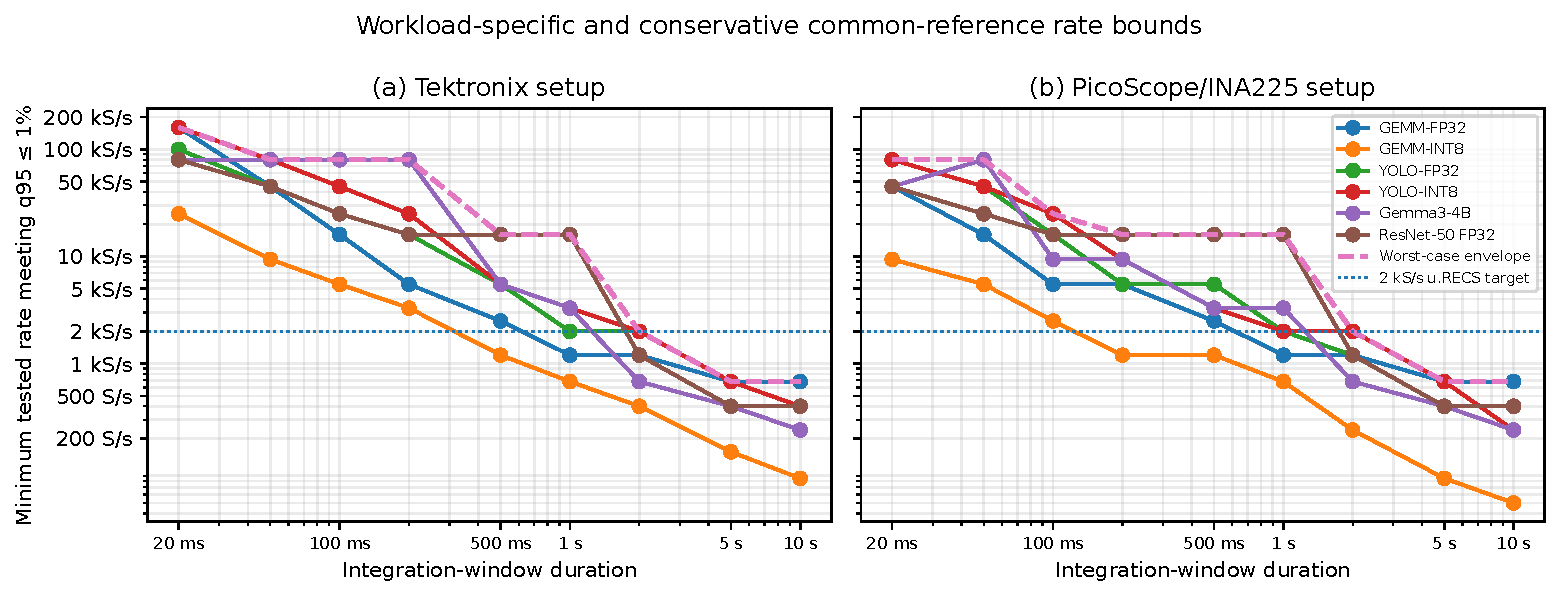
\includegraphics[width=\textwidth]{paper_artifacts/figures/cross_workload_fmin_paper.pdf}
  \caption{Workload-specific minimum tested rates for the 1\% energy criterion. A rate is reported only when that rate and every higher tested rate satisfy the criterion; the dashed curve is the maximum across available workloads and the dotted line marks the 2-kS/s u.RECS target.}
  \label{fig:cross-workload-fmin}
\end{figure}

\begin{figure}[t]
  \centering
  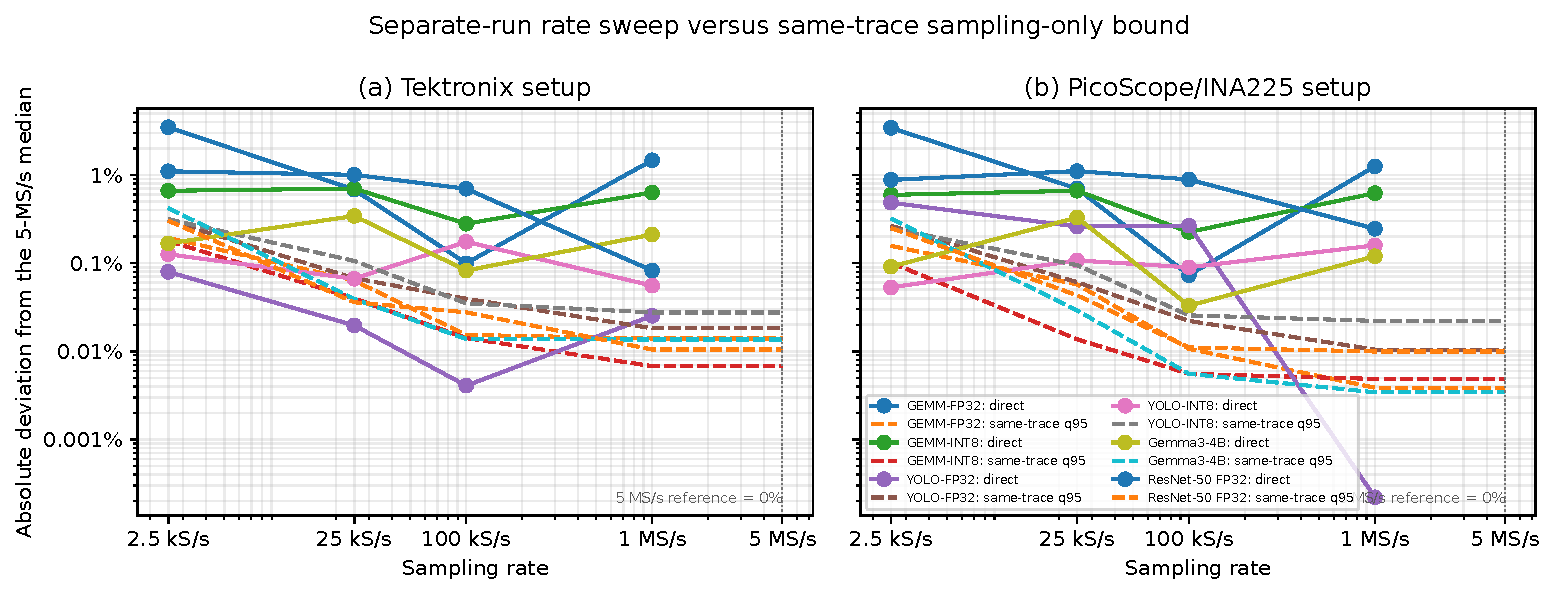
\includegraphics[width=\textwidth]{paper_artifacts/figures/cross_workload_direct_vs_common_reference_paper.pdf}
  \caption{Separate-run rate-sweep deviations versus same-trace sampling-only bounds. Solid curves show deviations of independently acquired runs from the 5-MS/s median; dashed curves show the q95 bound reconstructed from the same physical trace. The 5-MS/s zero reference is annotated rather than displaced on the logarithmic axis.}
  \label{fig:cross-workload-direct}
\end{figure}
